\chapter{Background}
\label{chp:background}

\section{Why We Need Incident Management}
\label{sec:threatLandscape}
Modern society shows an increasing use of digital solutions. Today, digital solutions are vital to most organizations' day-to-day operations and large amounts of sensitive data are stored digitally \cite{KriposTrender}. As the value and sensitivity of information increases, the number of potential threats increase accordingly. This suggests that organizations today are more exposed to attacks than before. This section discusses the current threat landscape and the need for plans in situations where systems have not been sufficiently secure. 

Organizations are increasingly using and depending on information technology in their operations. Attacks get more advanced and attackers choose their targets more strategically. A significant challenge arises when new and severe security threats evolve faster than corresponding measures. This leads to an increasing gap between threats and security measures in organizations. To avoid severe consequences such as disclosure of sensitive information, this gap must be closed.

Despite organizations' implementation of information security policies and controls, it is inevitable that new vulnerabilities and information security incidents occur occasionally. Thus, it is essential that organizations have a structured and planned approach to detect, report, assess, respond to and learn from information security incidents \cite{ISO/IEC27035}. Preventive actions are not sufficient and an incident management capability is therefore necessary.

\begin{newquote}{Roar Thon, Senior Adviser \acs{NSM}}
\textit{"Everybody should do what they can to protect themselves from being attacked, but the sad truth is that the most important thing you should plan and prepare for is how to behave when the attacker has succeeded"}
\end{newquote}

The information security threat landscape is continuously changing and new types of security-related incidents emerge frequently \cite{nist800-61}. %Preventive actions are not sufficient in order to be able to handle this and an incident response capability is therefore necessary. Even though incident prevention is not sufficient, it is an important complement to incident response. 

\acs{NSM} \acs{NorCERT}\footnote{\acs{NSM} is the Norwegian National Security Authority and is a cross-sectional professional and supervisory authority within the protective security services in Norway \cite{AboutNSM}. \acs{NorCERT} is the \acl{NorCERT} and is part of \acs{NSM}. \acs{NorCERT} coordinates preventive work and responses against IT security breaches aimed at vital infrastructure in Norway \cite{AboutNorCERT}} has registered a 30\% increase in cases each year for the past few years. They have seen an increase in cases of all impact levels. In addition they believe that there is a large number of incidents not reported or discovered \cite{NorCERT3Kvartal2012}. These findings are supported by Kripos\footnote{Kripos is the \ac{NCIS} in Norway and it is the unit for combating organized and other serious crime \cite{policeInNorway}.}, that reports ICT related crime to be expanding \cite{KriposTrender}. There is a large increase in targeted espionage operations directed towards Norwegian industry \cite{NSMRapport2012}. Attacks are mainly driven by \ac{ROI}, thus targets are chosen based on potential profit. Other incidents not necessarily motivated by money are strategic targets and domestic political monitoring as seen in China and Syria\cite{Morketall2012}.

\acs{NSM} states that the security condition in Norway for 2012 is not satisfactory \cite{samordnaVurdering}. This seems to be a continuing trend and the security condition for 2011 was summarized in the following way \cite{NSMRapport}: 

\begin{quote}
\textit{``The \textbf{values} we want to protect increase in amount, the \textbf{threats} are increasing, new \textbf{vulnerabilities} are constantly discovered, but \textbf{measures} to reduce these vulnerabilities are not developed at the same rate in addition to being inadequate."}
\end{quote}

Additionally, there is an increasing number of vulnerabilities discovered on smart phones and tablets, which represents a relatively new part of the threat landscape. There exist persistent vulnerabilities in organizations with classified information and these exist mainly due to lack of understanding of risks \cite{NSMRapport2012}.

In 2012 \acs{NorCERT} handled a large amount of serious cases related to espionage against Norwegian high-technology organizations \cite{NorCERT3Kvartal2012}. In a recent report PST\footnote{The Norwegian Police Security Service} expressed concerns related to Norwegian research and education environments being exploited to strengthen other nations' defences \cite{PSTvurdering2013}.   

Many of the current threats cannot be stopped by antivirus software. Attacks are increasingly becoming targeted to specific organizations in addition to becoming more advanced. Delay in updates and patches of computers is a big problem for many organizations \cite{NorCERT2Kvartal2012}. \acs{NSM} has observed a change in attacks from random and opportunistic attacks to advanced and focused attacks on specific targets of high economic or social value. In addition to technical means, attackers use social engineering\footnote{Social engineering involves manipulating people into performing certain actions such as disclosing sensitive information.} to obtain sensitive information or to obtain access to systems \cite{NSMRapport}. Another trend is attacks that compromise legitimate websites and infect all users that visit them \cite{NSMRapport2012}. Such attacks are called water-holing. They are particularly difficult to protect against as these exploit websites that users are normally allowed to visit.

There is great diversification in type of attackers. Attackers can belong to foreign intelligence, traditional military, global businesses, terrorist organizations, hacker groups or they can operate individually \cite{samordnaVurdering}. Criminals are organized in new ways, and various participants contribute with services, making attacks possible \cite{KriposTrender}. It is even possible to buy attacks like \ac{DDoS} attacks or spam distribution \cite{NorCERT2Kvartal2012}. Attacks can also come from the inside, either from an insider or by social engineering, and many organizations do not focus on this threat \cite{NSMRapport2012}. This expands the group of possible attackers, in practice it includes everyone. 

Several publications and recent reports highlight the need for incident management by pointing out deficiencies in organizations' information security. PST states that information security is given low priority in Norwegian government and private institutions \cite{PSTvurdering}. This is supported by \acs{NSM} that states that organizations seem to lack the ability and/or will to prioritize ICT-security \cite{NSMmelding}. Incident handling is often not prioritized and the severity of attacks are often not understood \cite{NorCERT2Kvartal2012}. Management's knowledge of information security is often insufficient, which is unfortunate as this is key to commitment of the rest of the organization \cite{NorCERT3Kvartal2012}. Systems for reporting security incidents to the management rarely exist and \acs{NSM} almost always discover that incidents have occurred or are occurring when they perform inspections\cite{NSMRapport}. Many organizations have inadequate contingency plans related to information security. Organizations also omit to conduct rehearsals related to preventive security and omit to rehearse their contingency plans \cite{NSMRapport2012}.

Several trends described here are not unique to Norway. Verizon Enterprise's RISK team published a report in cooperation with the \ac{USSS}, the Dutch \ac{NHTCU}, the \ac{AFP}, the \ac{IRISS} and the \ac{PCeU} of the London Metropolitan Police \cite{VerizonReport}. The report discusses data breaches in 2011 in 36 different countries. 855 incidents were analysed. It shows that 96\% of the (reported) attacks were not particularly advanced. It also shows that 85\% of the breaches took weeks or more to discover and that 92\% of incidents were discovered by a third party. 86\% of the breaches were caused organized crime. Based on the cases reported to the involved organizations, 2011 seems to be the year with the second highest number of data losses since 2004. The results of this report indicate that the overall international security condition is not satisfactory.

This shows a complex threat landscape with a large variety of attackers and with organizations that are not sufficiently prepared. It is not realistic to believe that all incidents can be prevented. In addition, it is not economically feasible. Hence, it is evident that organizations need plans and procedures to handle incidents \textit{when} they occur. The existence of an incident response capability in an organization can assist them in rapidly detecting incidents, minimizing loss and destruction, mitigating the weaknesses that were exploited and restoring computing services \cite{nist800-61}. 

\section{Incident Management Overview}
%Eller noe i den duren, måtte bare ha en section til subsectionen :p
\subsection{Definitions}
\label{sec:Definitions}
%Eller et annet navn, poenget er å includere definisjoner av disse tidlig i rapporten
In information security incident management there are a few terms that need to be defined clearly. Two such terms are information or computer security incidents\footnote{In this report the terms ``information security incident", ``computer security incident" and ``incident" are used interchangeably.} %NB! På slutten, sjekk at dette faktisk stemmer!
and information or computer security events. It is important to recognize these as two terms of different meaning. The standard \acs{ISO}/\acs{IEC} 27000 \cite{ISO/IEC27000} specifies the following definitions:

\textbf{Information security:} Preservation of confidentiality, integrity and availability of information; in addition, other properties such as authenticity, accountability, non-repudiation and reliability can also be involved.

\textbf{Information security event:} Identified occurrence of a system, service or network state indicating a possible breach of information security policy or failure of safeguards, or a previously unknown situation that may be security relevant.

\textbf{Information security incident:} Single or a series of unwanted or unexpected \emph{information security events} that have a significant probability of compromising business operations and threatening information security.

\textbf{\ac{ISIRT}:} Team of appropriately skilled and trusted members of the organization that handles information security incidents during their lifecycle.

The guidelines \acs{NIST} SP 800-61 \cite{nist800-61} specifies the following definitions:

\textbf{Event:} An event is an observable occurrence in a system or network.

\textbf{Adverse event:} Adverse events are events with a negative consequence, such as system crashes, packet floods, unauthorized use of system privileges, unauthorized access to sensitive data, and execution of malware that destroys data.

\textbf{Computer security incident:} A violation or imminent threat of violation\footnote{An ``imminent threat of violation" refers to a situation in which the organization has a factual basis for believing that a specific incident is about to occur.} of computer security policies, acceptable use policies, or standard security practices.

\acs{NorCERT} specifies the following definitions \cite{NorCERT3Kvartal2012}:

\textbf{\ac{CSIRT}:} A central tool with the task of protecting important infrastructure. The team must consist of security specialists and they must handle and responds to incidents. Additionally they need to create awareness and educators.

\textbf{\ac{CERT}:} A trademark that can only be used after approval by Carnegie Mellon University. Is in practice the same as a \acs{CSIRT}.

The definition of an adverse event from \cite{nist800-61} is quite similar to the definition of information security event from \cite{ISO/IEC27000}. The definitions of incidents are also quite similar. These definitions are the ones that will be used in this report. \ac{ISIRT}, \ac{CSIRT} and \ac{CERT} define similar types of teams. In this report the term \acs{IRT} is used to denote such a team. 

\subsection{What is Incident Management}
Incident management is a collective term composing all activities associated with managing security incidents. Incident management is not restricted to incident response but includes activities for the entire incident lifecycle; from planning, training and raising awareness to detecting, responding and learning from incidents. 

Various guides and standards describe best practice and suggest activities for effective and efficient incident management. It is important to note that incident response requires a substantial amount of planning and resources. Some of the most important parts of incident response are the existence of guidelines for communication and prioritization of incidents as well as the use of a lessons learned process to gain experience from incidents. \cite{nist800-61}

As part of an incident management capability, organizations should have an incident response policy, an incident response plan and incident response procedures, all of which should be tailored to the specific organization's needs. Additionally it is important to have a planned approach to reporting of vulnerabilities that have not yet been exploited \cite{ISO/IEC27035}.

%The policy should include definitions, forms and commitment from senior management, plans should outline the organization's approach towards incident response, whereas procedures should be based on the current incident management policy and plan.

%\acp{SOP} are a delineation of the specific technical processes, techniques, checklists and forms used by the incident response team. An organization should establish procedures regarding communication with various outside parties, like media, law enforcement, other incident response teams, software vendors and \acp{ISP}. It is common to have \acp{PoC} for the various outside parties. \cite{nist800-61}

Incident management is not purely an IT issue, because incidents threaten an organization as a whole. Incident management seeks to prevent, contain and resolve incidents, in addition to learning from them in order to improve current procedures. ``Thus, incident management is an important tool of overall governance and to have it, in whatever form or shape, is a necessity\cite{enisaGuide}." 

\subsection{\acl{IRT}}
Despite extensive preparation and security implementations, incidents occur occasionally. Thus, organizations need incident response to mitigate damage caused by compromised personal or confidential information. Having an \ac{IRT} will aid organizations in responding to incidents more effectively and efficiently, in addition to providing a structured approach for learning from previous incidents. 

As the various definitions of response teams indicate in \ref{sec:Definitions}, an \ac{IRT} ``is a team that responds to computer security incidents by providing all necessary services to solve the problem(s) or to support the resolution of them\cite{enisaCSIRTGoodPractices}." \ac{IRT} structure, members, tasks and responsibilities may vary depending on organizations' resources and need for information security. 

All organizations relying on IT should have an incident response team available to handle incidents. Large organizations may choose to have several incident response teams, e.g. one team per division. The structure of the team may vary and can be dedicated, virtual or a mix of the two. However, the ISO/IEC 27035 standard recommends having a permanent team. \acp{IRT} should have clearly defined responsibilities, processes, allocation of roles and appropriate training programs\cite{ISO/IEC27035}. 
Team members should hold appropriate access permissions, have access to supportive tools to be best possibly prepared to conduct incident response \cite{SANShandbook}.

\ac{NIST} recommends having one person in charge of incident response, taking the role as team manager. The team manager should act as a liaison to senior management as well as ensuring that the team has the necessary resources, personnel and skills. It is recommended that team members have diverse backgrounds so they are able to handle different incidents that may arise. Usually teams consist of highly technically skilled persons, and teams should have at least one member with experience in each major technological category. However, it is not required that \emph{all} team members are technical experts. Nevertheless, good problem solving skills and communication skills are important since effective and efficient incidents response require collaboration and coordination within the team and throughout the organization.

To minimize the frequency of incidents and to mitigate negative impact caused by them, most \acp{IRT} do not \emph{only} provide reactive services, but may also have other responsibilities, such as intrusion detection, advisory distribution, education and raising awareness within the organization\cite{nist800-61}. 
 

%The mission of the \ac{CERT} should reflect what is really important for the organization. The \ac{CERT} must define its constituency. The constituency is the organization or group of organizations and/or people whose incident the team handles. \cite{enisaGuide}  

\section{Standards and Guidelines}
\subsection{The \acs{ISO}/\acs{IEC} 27001 Standard}
\label{sec:iso27001}
This standard provides a model for establishing, implementing, operating, reviewing, maintaining and improving an \ac{ISMS}. It states that management shall provide evidence of its commitment to the ISMS. This section presents clauses relevant to incident management that are directly retrieved from the standard \cite{ISO/IEC27001}. 

\textbf{4.2.2 Implement and operate the \ac{ISMS}} \\
The organization should do the following.
\begin{enumerate}[h)]
\item Implement procedures and other controls capable of enabling prompt detection of security events and response to security incidents.
\end{enumerate}

This clause specifies that organizations should be able to detect and handle security incidents.

\textbf{4.2.3 Monitor and review the ISMS}\\
The organization shall do the following.
\begin{enumerate}[a)]
\item Execute monitoring and reviewing procedures and other controls to:
\begin{enumerate}[2)]
\item promptly identify attempted and successful security breaches and incidents;
\end{enumerate}
\vspace{-0.2cm}
\begin{enumerate}[4)]
\item help detect security events and thereby prevent security incidents by the use of indicators;
\end{enumerate}
\vspace{-0.2cm}
\begin{enumerate}[5)]
\item determine whether the actions taken to resolve a breach of security were effective.
\end{enumerate}
\item Undertake regular reviews of the effectiveness of the \ac{ISMS} (including meeting \ac{ISMS} policy and objectives, and review of security controls) taking into account results of security audits, incidents, results from effectiveness measurements, suggestions and feedback from all interested parties.
\end{enumerate}

\textbf{4.3.3 Control of records}\\
Records shall be kept of the performance of the process as outlined in 4.2 and of all occurrences of significant security incidents related to the \ac{ISMS}

Common for all clauses in this standard is that they only specify that things should be done, and not \textit{how} they should be done. The \acs{ISO}/\acs{IEC} 27002 standard\footnote{ \acs{ISO}/\acs{IEC} 27002 Information technology - Security techniques
- Code of practice for information security management} provides a code of practice for information security management and the \acs{ISO}/\acs{IEC} 27035 standard provides guidelines for the establishment of information security incident management. These standards are further described in sections \ref{sec:iso27002} and \ref{sec:iso27035} and can be used as aids to fulfil the clauses presented in the \acs{ISO}/\acs{IEC} 27001 standard.
\subsection{The \acs{ISO}/\acs{IEC} 27002 Standard}
\label{sec:iso27002}
This standard represents a code of practice for information security management and establishes guidelines for initiating, implementing, maintaining and improving information security management in an organization. The standard is intended to be a starting point for developing organization specific guidelines and contains 11 security control clauses that outline various security objectives and provide implementation guidance. It is emphasized that organizations should initially identify and establish their security requirements and then choose which of the security controls to implement.

This section presents clauses from the standard that are relevant to incident management. They are retrieved from \cite{ISO/IEC27002}.

\textbf{13.1 Reporting information security events and weaknesses } \\
The objective is to ensure that all significant information security events and weaknesses are reported such that corrective actions can be made in time. Reporting procedures and employee awareness are important success factors and it should be required to report any events or weaknesses to the point of contact as quickly as possible.

\textbf{13.1.1 Reporting information security events} \\
\emph{Control:} Information security events should be reported through appropriate management channels as quickly as possible.

\emph{Implementation guidance:} A point of contact and a formal event reporting procedure should be established and employees should be made aware of these. The reporting procedure should include the following.
\begin{enumerate}[a)]
\item suitable feedback processes to ensure that those reporting information security events are notified of results after the issue has been dealt with and closed.
\item information security event reporting forms to support the reporting action, and to help the person reporting to remember all necessary actions in case of an information security event.
\item the correct behaviour to be undertaken in case of an information security event.
\item reference to an established formal disciplinary process for dealing with employees, contractors or third party users who commit security breaches.
\end{enumerate}

\textbf{13.1.2 Reporting security weaknesses} \\
\emph{Control:} All employees, contractors and third party users of information systems and services should be required to note and report any observed or suspected security weaknesses in systems or services.

\emph{Implementation guidance:} There should exist an easy, accessible and available reporting mechanism for employees, contractors and third party users. Weaknesses should be reported as quickly as possible to either management or the service provider and not attempted to be proven.

\textbf{13.2 Management of information security incidents and improvements}\\
The objective is to ensure that the management of security incidents follows a consistent and effective approach where responsibilities and procedures are in place to handle incidents once they have been reported. Procedures should be in place for continual improvement of management processes. When necessary to collect evidence, this should be done in compliance with legal requirements.

\textbf{13.2.1 Responsibilities and procedures}\\ 
\emph{Control:} Management responsibilities and procedures should be established to ensure a quick, effective and orderly response to information security incidents.

\emph{Implementation guidance:} In addition to reporting, monitoring should be used to discover incidents. When implementing incident management procedures organizations should consider the following.
\begin{enumerate}[a)]
\item procedures should be established to handle different types of information security incidents, including:
\begin{enumerate}[1)]
\item information system failures and loss of service.
\item malicious code.
\item denial of service.
\item errors resulting from incomplete or inaccurate business data.
\item breaches of confidentiality and integrity.
\item misuse of information systems.
\end{enumerate}
\item in addition to normal contingency plans, the procedures should also cover:
\begin{enumerate}[1)]
\item analysis and identification of the cause of the incident.
\item containment.
\item planning and implementation of corrective action to prevent recurrence, if necessary.
\item communication with those affected by or involved with recovery from the incident.
\item reporting the action to the appropriate authority.
\end{enumerate}
\item audit trails and similar evidence should be collected and secured, as appropriate, for:
\begin{enumerate}[1)]
\item internal problem analysis.
\item use as forensic evidence in relation to potential breach of contract or regulatory requirement or in the event of civil or criminal proceedings, e.g. under computer misuse or data protection legislation.
\item negotiating for compensation from software and service suppliers.
\end{enumerate}
\item action to recover from security breaches and correct system failures should be carefully controlled. The procedures should ensure that:
\begin{enumerate}[1)]
\item only certain identified and authorized personnel are allowed access to live systems and data.
\item all emergency actions taken are documented in detail.
\item emergency action is reported to management and reviewed in an orderly manner.
\item the integrity of business systems and controls is confirmed with minimal delay.
\end{enumerate}
\end{enumerate}

\textbf{13.2.2 Learning from information security incidents}\\
\emph{Control:} There should be mechanisms in place to enable the types, volumes, and costs of information security incidents to be quantified and monitored.

\emph{Implementation guidance:} By monitoring incidents, reoccurring and high impact incidents can be identified and need for additional controls can be evaluated.

\textbf{13.2.3 Collection of evidence}\\
\emph{Control:} Where a follow-up action against a person or organization after an information security incident involves legal action (either civil or criminal), evidence should be collected, retained, and presented to conform to the rules for evidence laid down in the relevant jurisdiction(s).

\emph{Implementation guidance:} The rules of evidence involve admissibility and weight of evidence, that is whether or not evidence can be used in court and the quality and completeness of the evidence. To achieve admissibility and weight of evidence, organizations should ensure their systems comply with standards and that controls used to protect evidence are complete and consistent.

\subsection{\acs{ISO}/\acs{IEC} 27035}
This section gives an introduction to the ISO 27035 standard and the content is, unless specified otherwise, derived from \cite{ISO/IEC27035}. 

Implementing this standard will aid organizations in dealing with information security incidents properly and mitigate both direct and indirect adverse business impact. This standard provides an extensive and structured approach towards incident management by presenting five phases with recommended activities for large and medium-sized organizations. 

One of the standard's objectives is to provide guidelines to aid organizations in meeting the requirements specified in ISO/IEC 27001. %For this purpose a cross-reference table showing how following the guidelines in ISO/IEC 27035 fulfils the requirements in ISO/IEC 27001 is given in the appendix.

\paragraph{Plan and Prepare} This phase is by far the most extensive phase and involves many activities. Individual organizations have to ensure that their use of resources are proportional and according to their needs. Each organization should formulate an incident management policy reviewing current vulnerabilities, stating the need for an incident management scheme and identifying overall benefits for the organization. Security and risk management policies should be reviewed and updated regularly. The standard highlights the importance of ensuring commitment from senior management in the security incident management policy to ensure the organization's commitment to resources and maintenance of an incident management capability.  

One main activity in the plan and prepare phase is making a detailed incident management scheme that contains forms, procedures and support tools for the detection and reporting of, assessment and decision making related to, making responses to and learning lessons from incidents. The scheme should include a classification scale for grading incidents and reporting forms (preferably electronic).   

An important activity in this phase is the establishment of the \acf{ISIRT}. Organizations should also establish and implement required mechanisms of support for their incident management scheme to operate efficiently during this phase. This includes technical tools such as IDS and log monitoring systems as well as relationships and connections to other organizations. 

It is essential for the success of a structured incident management approach that awareness and participation of all personell is present. All personell should be familiar with the incident management scheme when it comes operational and be able to recognize its benefits. It is therefore recommended that an appropriate awareness and training program is developed and repeated from time to time as personell change over time.

The entire incident management scheme should be tested to verify that the scheme and \ac{ISIRT} work in complex and real situations. When this phase is completed, organizations should be fully prepared to manage security events, incidents and vulnerabilities that occur.

\paragraph{Detection and Reporting} The first operational phase of an incident management scheme involves detection, collection of information and reporting of occurrences of security events, incidents and vulnerabilities either discovered by humans or automated systems. It is important to preserve information about vulnerabilities and incidents in a database operated and maintained by the \ac{ISIRT}. Organizations should implement security monitoring systems, \acl{IDS}/\acl{IDP} (\acs{IDS}/\acs{IDP}), antivirus programs and so forth to aid the detection of security events, incidents and vulnerabilities. Logs from various entities should be analysed and registrations of incidents should be made in an Incident Tracking System. 

It is the person first notified about an event that is responsible for starting the activities involved in this phase. There are several ways a security event or incident can be discovered and thus all personell should be aware of and have access to the guidelines for reporting. There should be clear procedures to follow for the people involved in dealing with an incident. All relevant information should be passed to the PoC and the responsible \ac{ISIRT} member. It is recommended that one of the \ac{ISIRT} members are appointed the responsibility for incoming reports and makes an assessment for further actions.  A reporting form should be specified to ensure that all necessary and relevant information is preserved and that there is consistency in information gathered. 

\paragraph{Assessment and Decision} This phase includes assessment of information regarding security events and decisions on whether events should be treated as incidents. The assessment and decision phase also includes assessment of information received regarding vulnerabilities and decisions of how to handle these in accordance with previously agreed actions.

The PoC should use a predefined classification scale to make an assessment of security events, whether they are incidents or false alarms and what impact they may have on the organization's core services, information and affected assets. The initial assessment made by the PoC should be verified by an \ac{ISIRT} member. \ac{ISIRT} makes decisions about how the incident should be handled, by whom and in what priority. To be able to respond to security incidents in an efficient and effective way, a prioritizing process should be conducted based on the level of adverse business impact and the required effort to solve them.  All information pertaining to an incident should be recorded in the database by \ac{ISIRT}. A main activity for the \ac{ISIRT} is to allocate responsibilities for incident management actions and provide thorough and structured procedures for persons involved to follow. 

\paragraph{Responses} The third operational phase presents guidelines and activities for organizations in responding to security incidents. The response should be in accordance with the actions agreed in the previous phase, whether it is an immediate, real-time or near real-time response or involves forensics analysis. This phase also involves making responses to vulnerabilities reported either internally or by other parties. As a first step the \ac{ISIRT} has to determine whether the incident is under control, and then initiate the appropriate actions. For situations out of control, escalation to crisis handling might be necessary for further assistance. Otherwise, the response work such as recovery, proper documentation and communication to relevant parties can be started. 

The \ac{ISIRT} should consider which internal and possibly external resources to utilize for best responding to incidents. It is important that every action conducted by the \ac{ISIRT} in this phase is logged properly and that guidelines are used to ensure thorough documentation. Logging actions will aid in analysing how effective and efficient the incident response process was as well as ensuring that any possible evidence is not compromised. It is the \ac{ISIRT}'s responsibility to make sure the affected assets become operational again and that they are not vulnerable to the same attack. Once an incident has been handled successfully, the case should be closed formally by the \ac{ISIRT} and recorded in the database.

\paragraph{Lessons Learned} The final phase starts after an incident has been resolved and/or closed and focuses on analysing whether the organization's incident management scheme worked successfully. During this phase improvements are identified and made. One of the main activities is reviewing how effective the entire incident management process was in responding to, assessing and recovering from the incident. Shortcomings and improvements in policies, procedures, security control implementations, reporting formats and risk assessments should be identified during this phase. Improvements may be implemented immediately or incorporated into future plans. The \ac{ISIRT} should make sure improvements are made to the entire system and not only the affected parts.

The lessons learned phase has many iterative activities. An essential post-incident activity is documenting incidents properly, ensuring incident trend analysis is accurate. Sharing experiences with trusted communities and partners should be done on a regular basis, regardless of whether incidents occur internally. Reviews, trend analysis and testing should be performed frequently to ensure regularly improvements to the incident response scheme over time. 





\subsection{\acs{NIST} Special Publication 800-61}
This subsection gives an introduction to the guidelines \acs{NIST} SP 800-61 and the content is, unless specified otherwise, derived from \cite{nist800-61}. This publication aims to  assist organizations in mitigating risks from computer security incidents by providing guidelines on how to respond to incidents effectively and efficiently. 

One of the first considerations for a \ac{CSIRC} should be to agree on a definition of the term incident. This guidelines' definitions of events and incidents are included in section \ref{sec:Definitions} of this report. 

\acs{NIST} SP 800-61 describes the four phases of incident response; preparation, detection and analysis, containment, eradication and recovery and post-incident activity. The phases and the relationship between them are illustrated in figure \ref{fig:NISTIncidentResponse}.

\begin{figure}[ht]
%\hspace*{-0.4cm}
\begin{center}
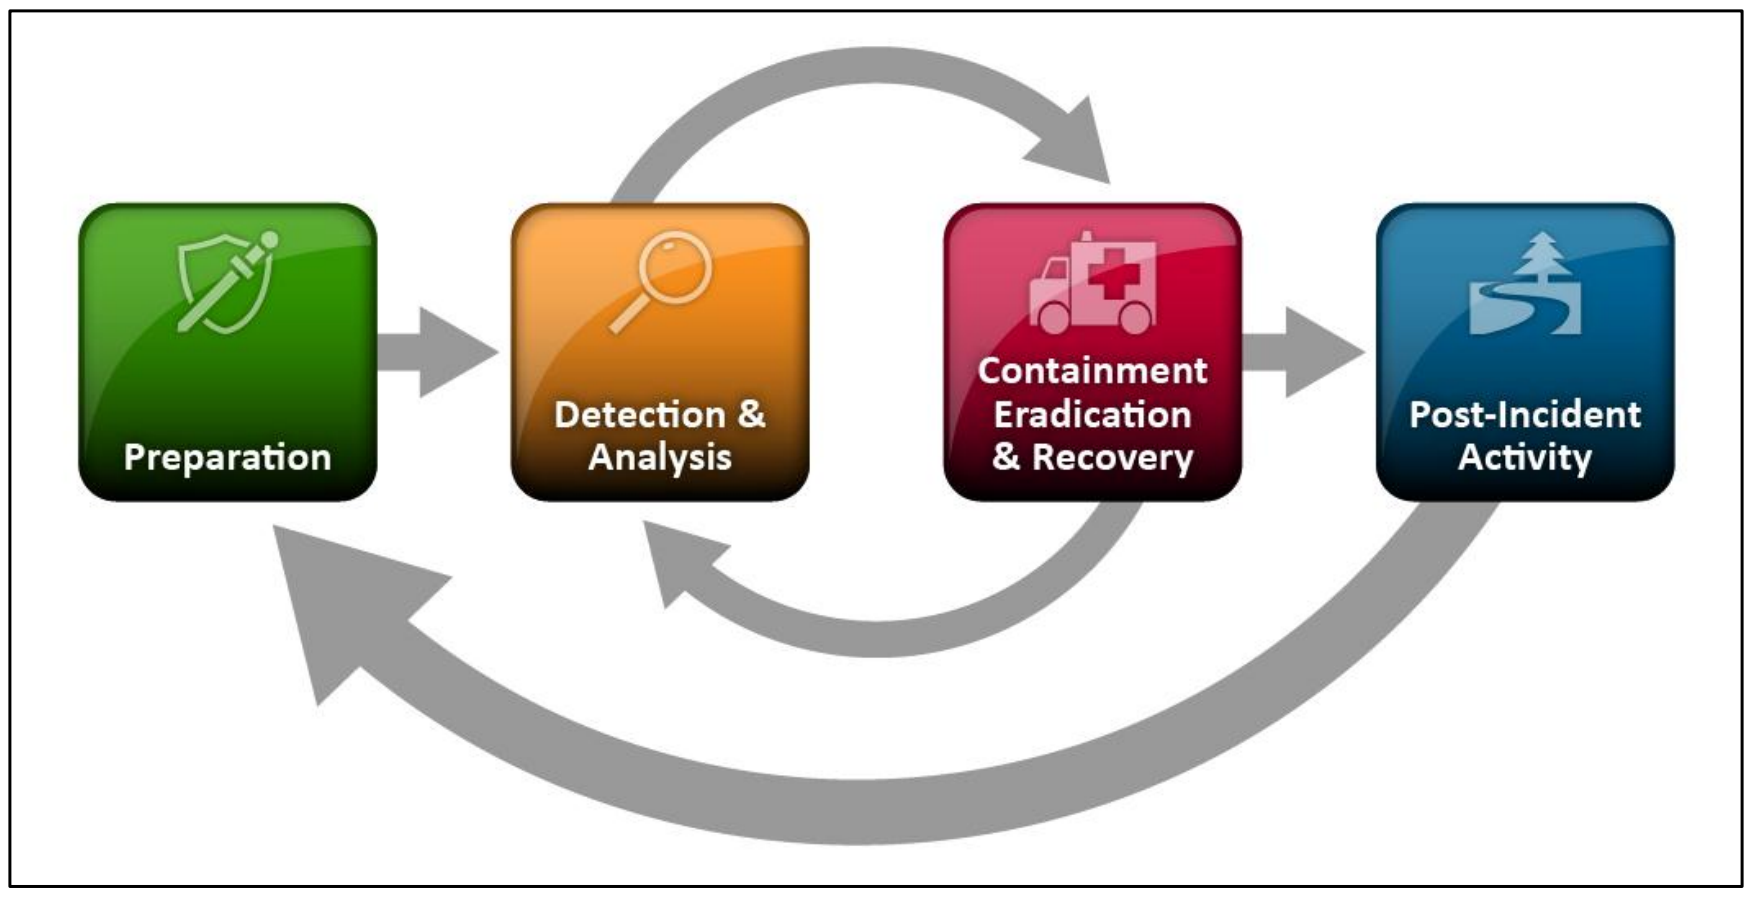
\includegraphics[scale=0.27]{NISTIncidentResponseCycle.png}
\caption[The Incident Response Life Cycle]{The Incident Response Life Cycle \cite{nist800-61}}
\label{fig:NISTIncidentResponse}
\end{center}
\end{figure}

\paragraph{Preparation} 
This phase includes establishing an incident response capability as well as preventing incidents. The latter is not typically a part of the incident response team's tasks, but it is fundamental to the success of the organization's incident response. If a large number of incidents occur, it may overwhelm the incident response team. To prepare for incidents the incident handlers should have tools and resources like contact information, incident reporting mechanisms, issue tracking system, digital forensic workstations\footnote{A digital forensic workstation is specially designed for acquiring and analysing data. It usually contains a set of removable hard drives that can be used for evidence storage.} and digital forensic software. It is common to create a portable \emph{jump kit} containing materials that may be needed during incident response.

\paragraph{Detection and Analysis}
Organizations should prepare to handle any type of incident and to handle common incident types. A classification of incidents can be used as a basis for incident handling. The guidelines provides a list of example categories for incidents that contains web, email, improper usage and loss or theft of equipment. This guidelines focuses on handling of any type of incident and not specific categories. A challenge related to incident handling is to detect the incident and determine the potential impact the incident may have. The actual detection may be the hardest part of incident handling. The guidelines defines two types of signs of incidents; precursors and indicators, with indicators being the most common. These are defined in the following way: "A \emph{precursor} is a sign that an incident may occur in the future. An \emph{indicator} is a sign that an incident may have occurred or may be occurring now." Common sources for precursors and indicators are \acp{IDPS}, antivirus and antispam software, third-party monitoring services, logs, information on new vulnerabilities and exploits and people. 

A challenging part of this phase is the analysis, i.e. to determine which indicators and precursors are legitimate, if they are really related to an incident and what has actually happened. When the team believes an incident to have occurred they should try to determine the scope. All steps taken should be documented and timestamped. It is important to note that any such documentation can be used in court. The incident response team should maintain a database containing information about incidents, such as status, indicators, related incidents and actions taken by the incident handlers. It is important to prioritize incidents and handle them accordingly. Factors that can be used as a basis for prioritization include the functional impact of the incident, the information impact of the incident and recovery from the incident. When the prioritization is performed the incident response team should notify the appropriate people. It is important to have procedures regarding who these people should be.

\paragraph{Containment, Eradication and Recovery}
Containment is obviously an important part of incident handling. The existence of strategies and procedures for containment is helpful. These strategies and procedures are different for different types of incidents. Gathering and handling of evidence is part of this phase. For some incidents eradication is necessary and for some it is done during recovery. Eradication can include deleting malware and disabling breached user accounts. Recovery consists of restoring systems to normal operation and in some cases eliminate vulnerabilities that could have causes similar incidents. The guidelines does not offer specific recommendations for eradication and recovery as these are often OS specific. 

\paragraph{Post-Incident Activity}
Learning and improving is one of the most important parts of incident response. It is recommended to hold a ``lessons learned" meeting after each major incident and periodically after lesser incidents. One meeting could cover several incidents. ``Lessons learned" meetings should generally focus on revealing what was done well and what could be improved. The desired result is that the organization will be better equipped for the next incident that occurs. Often incident response policies and procedures are updated. The areas these meetings should focus on include how well the staff performed and what they could have done differently, if documented procedures were followed and if they were adequate and how information sharing with other organizations could have been improved. To prevent future similar incidents potential corrective actions and potential additional tools and resources should be reviewed. Both people involved in the incident(s) in question and people needed for future cooperation should be included in these meetings. A follow-up report that provides a reference that can be used when handling future similar incidents should be created. Other post-incident activities include the use of collected data for risk assessment, measurement processes to determine the success of the incident response team and audits of incident response programs. 




\subsection{\acs{ENISA} - Good Practice Guide for Incident Management}
This guide is developed by the \ac{ENISA} and provides a description of good practices for security incident management. The content is, unless specified otherwise, derived from \cite{enisaGuide}. The focus of this guide is IT and information security incidents. It specifically addresses the incident handling part of incident management. The incident management and incident handling processes are illustrated in figure \ref{fig:ENISAIncidentManagement}. The incident handling process has four major components, as shown in the figure. 

\begin{figure}[h]
\begin{center}
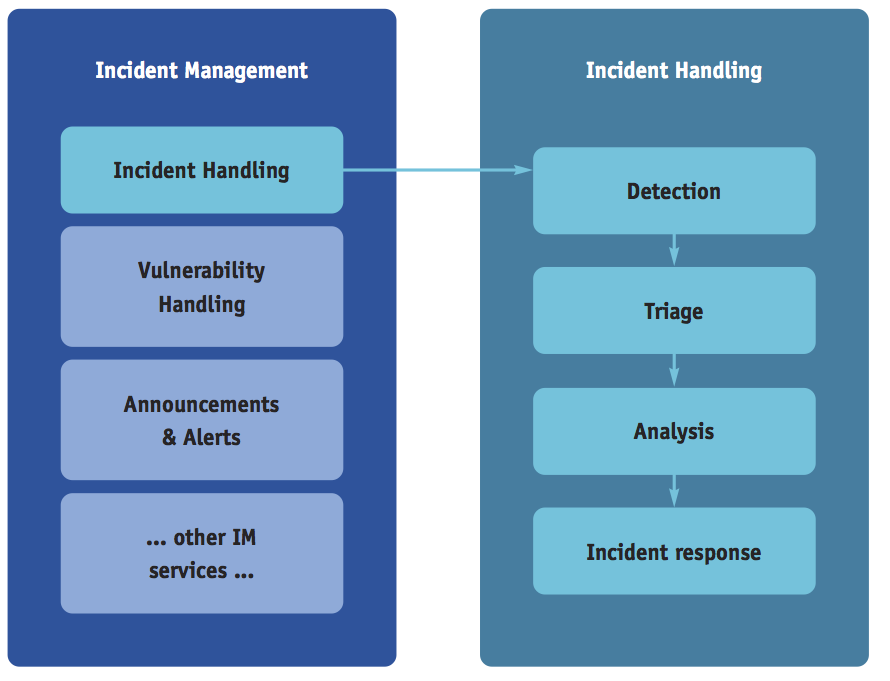
\includegraphics[scale=0.74]{enisaIncidentManagement.png}
\caption[ENISA Incident Management and Incident Handling]{Incident Management and Incident Handling \cite{enisaGuide}}
\label{fig:ENISAIncidentManagement}
\end{center}
\end{figure}

\paragraph{Detection:} The \ac{CERT} can receive incident reports from various sources. This guide recommends to use e-mail as a communication channel as people prefer this. Additionally, it recommends to use monitoring systems in addition to reports sent by others. Detection includes registration of incident reports in an incident handling system. This stage is a good place to implement pre-filtering mechanism for incident reports. The registration process could include the use of an incident report form.

\paragraph{Triage:} This stage consists of the three phases verification, initial classification and assignment. During these phases the following questions should be answered:

\begin{itemize}\itemsep-0.2cm
\item Is it really an IT security incident?
%\item Is it related to one of your constituents?
%\item Does it fit within the mandate the \ac{CERT} has?
\item What is the impact?
\item Is there collateral damage?
%\item How fast could it spread to other constituents?
\item How many people do you need to handle this incident?
\item Which incident handler should be appointed to the incident?
\end{itemize}

The verification phase seeks to answer the first question. It is however recommended to respond to and archive all reports, even those not defined as information security incidents. They may include information relevant to other incidents or potentially lead to an incident. After an incident report has been verified the incident should be initially classified according to a classification schema. The last part of the triage component is to assign the incident to an incident handler.

\paragraph{Analysis and Incident response:} These components are illustrated by figure \ref{fig:IncidentResolutionCycle}. The cycle may need to be iterated several times. To perform \textit{data analysis} there should be collected as much data as possible. Prior to the collection, all involved parties should be notified. Sources for data collection could be an incident reporter, monitoring systems, a referring database and relevant log files. The collected data should be used to try to determine the source of the incident. Prior to the data analysis, decisions about what data to analyse and in what order must be made. During the analysis, people will often exchange ideas and observations as well as draw conclusions. This belongs to the \textit{resolution research}. It is recommended to advise team members to write down any observations that can be discussed in review meetings. The \textit{action proposed} part consists of preparing a set of tasks for each party involved. The \textit{action performed} should be monitored, where possible. The main goal for all actions is the \textit{eradication and recovery}.

\begin{figure}[h]
\begin{center}
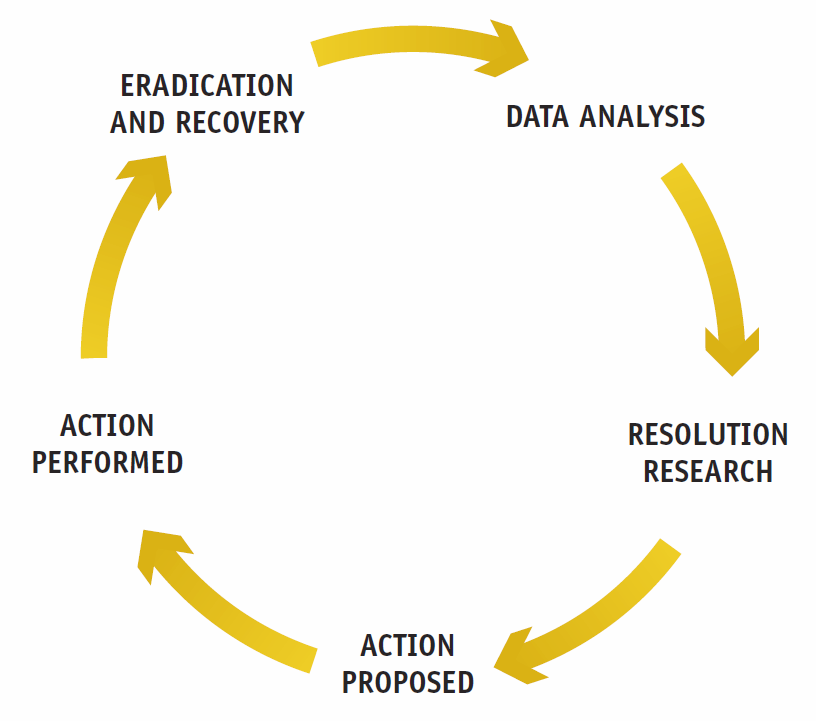
\includegraphics[scale=0.4]{IncidentResolutionCycle.png}
\caption[ENISA Incident Resolution Cycle]{Incident Resolution Cycle \cite{enisaGuide}}
\label{fig:IncidentResolutionCycle}
\end{center}
\end{figure}

When you have left the incident resolution cycle, there are still tasks to perform. The incident needs to be closed properly. Each involved party needs to be informed that the incident is resolved. The classification of the incident should be revisited and a final classification should be performed. The classification could have been revisited during the resolution cycle as well. It is recommended to have a taxonomy and to classify incidents in accordance with it.

After an incident has been resolved or closed a post-analysis should be performed in order to learn from the incident. It is also recommended not to analyse all incidents, but only the most characteristic and complex ones and those that include new attack vectors. 

Incidents should be reported to the management. In addition to specific issues, the daily operations should be reported, including costs, positive results, plans and risks. This will save time and resources in situations where you need the management's operational or financial support and quick decisions.





\subsection{NorSIS' Guideline for Incident Management}
The \ac{NorSIS} has in cooperation with a group of students\footnote{The students did a survey on incident management in Norwegian \acsp{SME}\cite{sand2010hendelseshaandtering}} developed a guideline for incident management, published in 2010\cite{norsisveiledning}. The aim of this guideline is to give a thorough description of why and how organizations should plan for security incident management, do business impact analysis and explain various measures to improve information security in organizations. The guideline distinguish between minimum requirements and general recommendations. The content in this section is, unless specified otherwise, derived from\cite{norsisveiledning}.

\paragraph{Incident Management Policy} 
An incident management policy should form the basis for developing new incident management plans in organizations. A solid policy should state an organization's objectives for incident management and include a statement ensuring commitment from senior management. Any relevant laws, standards and regulations should also be included. It is essential that the policy has requirements for performing regularly risk assessment, business impact analysis, tests and training. The guideline also suggests assigning roles and responsibilities as part of the incident management policy.

\paragraph{Business Impact Analysis}
NorSIS suggests that organizations conduct a business impact analysis to identify which services are of significant value and needs to be secured. Conducting risk assessment and identifying possible consequences of security incidents are part of this process. The guideline emphasize the importance of knowing risks and potential threats.  

\paragraph{Preventive Measures}
One of the most cost effective ways to do incident management is implementing preventive measures. Listed as minimum requirements are anti-virus, logs, firewalls, backups, alarms, locks, regularly reviews of threat landscape, and report systems for employees. Other proposed measures include encryption of data and wireless networks.   

\paragraph{Recovery Strategies}
The guideline recommends having a recovery strategy to quickly re-establish business operations after an incident. Suggestions include backup and emergency solutions. Routines and plans should be in place to handle recovery efficiently.

\paragraph{Incident Management Plan}
Organizations should use previous assessments and proposed incident scenarios to develop an incident management plan. It is recommended that individual plans addressing different scenarios are developed. Each incident management plan should state type of incident, what triggered the incident, roles and responsibilities, guidelines for communication and notification, maximum response time, check-list of tasks during incident response and post-incident activities.

\paragraph{Training}
To reduce costs caused by security incidents, NorSIS suggests training employees in correct use of equipment and make sure routines for incident response are well known.

\paragraph{Plan Maintenance}
The guideline recommends that organizations conduct yearly reviews of their incident management plans. To ensure a solid and up-to-date incident management plan, changes should be made based on experience from previous incidents. 

\paragraph{Outsourcing}
When organizations decide to outsource services, they should evaluate and agree on incident management procedures. It is the organization outsourcing that is responsible for securing information properly and to make sure sufficient plans for incident management exist. An agreement should define responsibilities and state expected quality of services. 

\paragraph{Example Threat Scenarios}
There should be no hesitations among employees when responding to typical threat scenarios. Examples of some security incidents are given and they aim to help organizations decide whether they have a sufficient incident management. Some examples are:
\begin{itemize}
\item Backup is lost due to a fire
\item The organization's network is attacked by a virus
\item There has been a burglary and two servers are stolen 
\end{itemize}

\subsection{SANS: Incident Handler's Handbook}
This section gives an introduction to the Incident Handler's Handbook and the content is, unless specified otherwise, derived from \cite{SANShandbook}. The purpose of this document is to provide sufficient information for IT-professionals and managers to create incident response policies, standards and teams for their organization. Six phases of incident response are described and recommended to be followed in sequence as each phase builds on the previous one. A check-list of relevant tasks for each phase, useful commands and areas to look for anomalous behaviour within both the Windows and UNIX environments are also included.

\textbf{Preparation} is the most crucial phase as it determines how well the incident response team will be able to respond to security incidents. During this phase, several key elements should be implemented to avoid potential problems while responding to security incidents.

Organizations should develop a policy stating the organization's principles, rules and practices. After establishing a security policy, organizations should organize a response plan with a prioritization of incidents based on organizational impact. Having this prioritization scheme could aid in getting necessary resources for incident management by ensuring commitment from senior management as they will better understand risk and business impact. It is also recommended having a communication plan so the response process is not delayed by uncertainty of whom to contact in unexpected situations. These plans should also state when it is appropriate to contact law enforcement.

Documenting incidents and the steps taken during incident response is extremely beneficial for organizations. A thorough documentation is useful for lessons learned and might also serve as evidence if an incident is considered a criminal act. As part of the preparation phase is the establishment of a \ac{CIRT}, and it is vital that also their activities are documented properly. 

\textbf{Identification} of security events by detecting deviation from ``normal" operations within the organization, followed by a decision of whether the event is categorized as an incident, are the first steps in the identification phase. Organizations should implement various tools to gather documentation about events, such that incidents and patterns can be identified. Examples of such tools include \acp{IDS}, firewalls and log files. Typically, incidents are reported to the \ac{CIRT} that decides the scope of the incidents and how to move forward with the next phase.

\textbf{Containment} is the next phase, where organizations try to limit the damage and prevent further damage caused by security incidents. It is recommended that compromised systems are isolated to avoid escalation, and an easy measure could be disconnecting affected parts of the system. 

This phase comprise several steps, all necessary for a successful incident response. The first step is called short-term containment and is concerned with limiting the damage by implementing short-term but effective solutions. The second step is ensuring proper back-up of information before system resources can be restored. The final step is long-term containment and involves removing alternations made by an attacker, installing security patches and limiting further escalation of the incident.

\textbf{Eradication} is the phase where affected assets and systems are restored. To avoid similar incidents from happening again, defences should be improved during this phase. Continuing documentation is important in this phase to ensure that proper steps were taken in previous phases as well as determining the overall impact to the organization. It is recommended that all affected systems are scanned with anti-malware software to ensure that all potential latent malware is removed. 

\textbf{Recovery} activities include bringing affected systems back into operation and preventing future incidents caused by the same problem as previous incidents. Other activities are testing, monitoring and validating systems to insure they are not reinfected. 

\textbf{Lessons Learned} is the final phase with main objectives to learn from incidents to improve the CIRT's performance and to provide materials to aid in response to future incidents. An important activity is holding a post-incident meeting summarizing the incident management process. This phase evaluates an organization's incident management procedures and identifies areas for improvement.

\section{Related Work}
Due to the increased focus on incident management in recent years, a few studies of organizations' practice exist. Unlike our research, most of the previous surveys are based on quantitative questionnaires.

A group of students at HiG\footnote{H\o gskolen i Gj\o vik (Norwegian)} did a survey of incident management policies, implementations, training and routines in Norwegian \acp{SME}. Their results indicate overall insufficient plans for incident management, and poor quality in existing plans. The survey focus on \acp{SME}  in a quantitative questionnaire, whereas our research focus on qualitative analysis of large organizations. Additionally, compliance with standards was not a focus in their studies, as is in ours.

In a quantitative study from 2005\cite{brage}, a survey of Norwegian companies and public institutions were performed to look at routines for security incidents, how theory and practice differ and difference between public and private institutions. Public institutions were found to have greater shortcomings in reporting, training and statistics than private companies. 